\chapter{Analisi e specifica dei requisiti}
\label{cap:Requisiti}
Nel presente capitolo si presenta il contesto nel quale il sistema andrà a lavorare, 
si analizzeranno le principali esigenze di un utente e, in termini generali, si mostrerà come il sistema risponde ed interagisce con l'utente. 

\section{Analisi Dominio}
Il  sistema  oggetto della tesi è un file system sviluppato per il nucleo didattico del Prof. Frosini e Prof. Lettieri, che verrà inserito nella versione SVN 568.\\
Il nucleo è diviso in tre moduli distinti, sia logicamente che in fase di linking, come di seguito sinteticamente mostrato : 
\begin{description}
 \item[Modulo Sistema]
  è il modulo principale del nucleo. In questo modulo vengono inizializzate le principali funzionalità di un kernel di cui sono importanti esempi la memoria virtuale e i processi.
  Questo modulo è in esecuzione con i privilegi di sistema. 
 \end{description}
 \begin{description}
  \item[Modulo IO]
  è il modulo nel quale vengono gestite le periferiche di input ed output. Anche questo modulo ha necessità dei privilegi Sistema per operare correttamente. 
  \end{description}
  \begin{description}
   \item[Modulo Utente]
  il modulo che gestisce i programmi utente. Questo modulo va in esecuzione con i privilegi utente. 
   \end{description}
Il file system per poter lavorare correttamente deve usare particolari istruzioni e/o strutture dati accessibili solamente dal livello sistema; si è perciò valutato opportuno inserire il file system nel modulo IO.\\ 
Tale scelta soddisfa anche la necessità di poter sfruttare tutte le potenzialità della memoria virtuale, necessaria per maneggiare le grandi strutture dati di cui è composto.

\section{Requisiti utente}
      In questa sezione analizziamo i requisti utente, cioè quello che l'utente si aspetta dal sistema. 
      L'applicazione deve fornire all'utente finale un file system funzionante compatibile con le specifiche del FAT32. Il file system deve mettere a disposizione delle funzionalità per la gestione dei file e delle cartelle da parte dell'utente.\\
      Più precisamente le specifiche dei requisiti per la gestione dei file sono : 
	\begin{enumerate}
	 \item L'utente deve poter creare ed eliminare i file;
	 \item L'utente deve poter scrivere e leggere  su un file;
	 \item L'utente deve poter stabilire la posizione all'interno del file dove effettuare le varie operazioni.
	\end{enumerate}
	
	Le specifiche dei requisiti per la gestione delle cartelle sono : 
	\begin{enumerate}
	 \item L'utente deve poter creare ed eliminare le cartelle.
	 \item L'utente deve poter navigare tra le cartelle.
	 \item L'utente deve poter ottenere la posizione corrente all'interno del volume. 
	\end{enumerate}
    
\section{Requisiti software}
\label{sez:Req}
    In questa sezione mettiamo in evidenza i requisiti software, cioè come il sistema soddisfa i requisiti utente.\\
    Il sistema deve fornire un metodo semplice per la gestione dei file e delle cartelle.
    Si è scelto di usare un approccio simile a quello usato nei sistemi unix basato sul concetto di\textbf{ descrittore di file} e \textbf{Path}. \\
      {\bf Definizione}: 
		\begin{quote}
		\textit{'Un descrittore di file (o file descriptor) è un numero intero non negativo che rappresenta un file  aperto da un processo e sul quale il processo può effettuare operazioni di input/output.'}
		\end{quote}
       {\bf Definizione}: 
		\begin{quote}
		\textit{'Il path di un file ( o cartella ) è un nome che contiene in forma esplicita informazioni sulla posizione del file all'interno del file system.'}
		\end{quote}

 Un file presente sul disco viene individuato in modo univoco dal path, e grazie a questa caratteristica un utente può svolgere le principali operazioni sul file.\\
 Ma per poter accedere al suo contenuto occorre creare un canale di comunicazione con il nucleo che renda possibile operare su di esso. 
 Questo è necessario perché i file risiedono sul disco, e questo risulta essere accessibile solamente mediante opportune routine di livello sistema del nucleo.\\
 Il canale di comunicazione si crea aprendo il file con la system call \textit{open} che inizializzerà tutte le strutture dati necessarie e restituirà il descrittore di file associato al file individuato dal path.
 Dopo aver aperto il file si avrà a disposizione il descrittore per effettuare le varie operazioni, ed una volta terminate queste, il canale di comunicazione si dovrà chiudere usando la \textit{close}. 
 All'interno di ogni processo i file aperti sono identificati dal descrittore di file. Questo approccio ha dei limiti, ogni processo può aprire un numero limitato di file ( configurabile ) senza che si creino malfunzionamenti a condizione che  nessun altro processo stia usando quel file. \\
 Tutta la gestione dei file avviene nel livello sistema del nucleo, quindi è stato necessario introdurre non semplici funzioni, ma system call\footnote { Una system call è il meccanismo usato da un processo a livello utente o livello applicativo per richiedere un servizio a livello kernel dal sistema operativo del sistema in uso.}
    che eseguano le richieste dell'utente effettuando anche il cambio di privilegio.\\
 Le cartelle presenti nel sistema possono essere gestite mediante l'interfaccia dei file, ma esistono alcune operazioni per le quali risulta necessario usare opportune system call per la loro gestione, in seguito metteremo in evidenza questa situazione. \\	
 Elenchiamo le system call per la gestione dei file: \\

    
     
     \begin{description}
      \item[Open]
	System call che apre il file e crea il canale di comunicazione con il nucleo .
     \end{description}
      
      \begin{description}
       \item[Close]
	System call effettua la chiusura di un file precedentemente aperto con open.
       \end{description}
       
       \begin{description}
        \item[Read] System call usata per leggere il contenuto di un file. Necessita che il file sia stato precedentemente aperto. 
	\end{description}

        \begin{description}
       \item[Write] System call usata per scrivere in un file.Necessita che il file sia stato precedentemente aperto. 
         \end{description}
     \begin{description}
      \item[Lseek] System call usata per spostare la posizione corrente del file.
      \end{description}
    
    \begin{description}
     \item[Remove] System Call usata per rimuove un file.
     \end{description}
     
     \begin{description}
      \item[Rename] System call che usata per rinominare un file.
      \end{description}
    
    \begin{figure}[h]
	\centering
	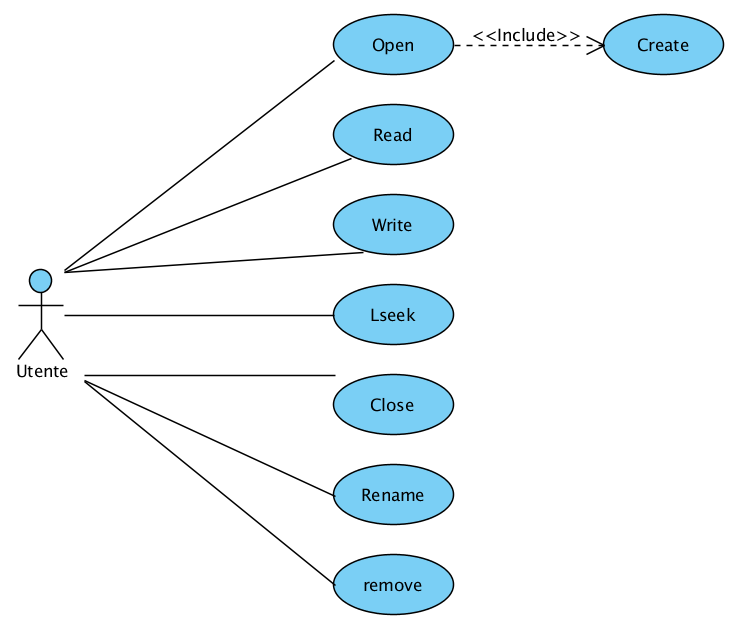
\includegraphics[width=300px,height=200px]{./Immagini/UseCaseFile.png}
	\caption{Diagramma Caso d'uso gestione File}
	\label{Fig.:UseCaseFile}
    \end{figure}

  \newpage

  Elenchiamo le system call per la gestione delle cartelle: \\

    \begin{description}
     \item[mkdir]System call utilizzata per creare una directory.
     \end{description}
     
     \begin{description}
      \item[rmdir]System call che elimina una directory. 
      \end{description}
      
      \begin{description}
       \item[chdir] System call che permette di cambiare la directory corrente. 
       \end{description}

      \begin{description}
     \item[getcwd] System call che riporta la directory corrente. 
    \end{description}

\begin{figure}[h]
 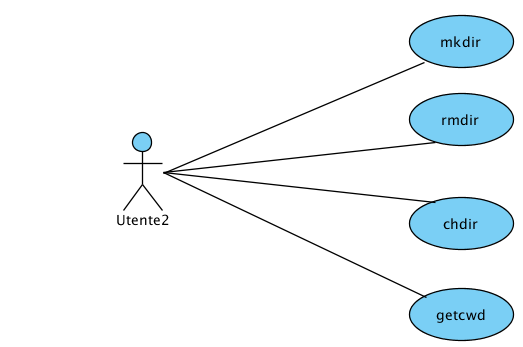
\includegraphics[width=300px,height=150px]{./Immagini/UseDir.png}
\caption{Diagramma Caso d'uso gestione Cartelle}
\end{figure}

\section{Conclusioni}
  In questo capitolo ho presentato i vari obiettivi che il sistema cerca di raggiungere. Nell'analisi dei requisiti software si è fatta un'introduzione molto semplice dell'architettura software, scegliendo di mettere in evidenza il punto di vista dell'utente. Un miglior dettaglio della struttura software è presentato nel capitolo §\ref{cap:Struttutra_Progetto}



\clearpage{\pagestyle{empty}\cleardoublepage}
